\documentclass{standalone}
\usepackage{tikz}
\usetikzlibrary{patterns, positioning}
\usepackage[sfdefault]{ClearSans} %% option 'sfdefault' activates Clear Sans as the default text font
\usepackage[T1]{fontenc}

\begin{document}
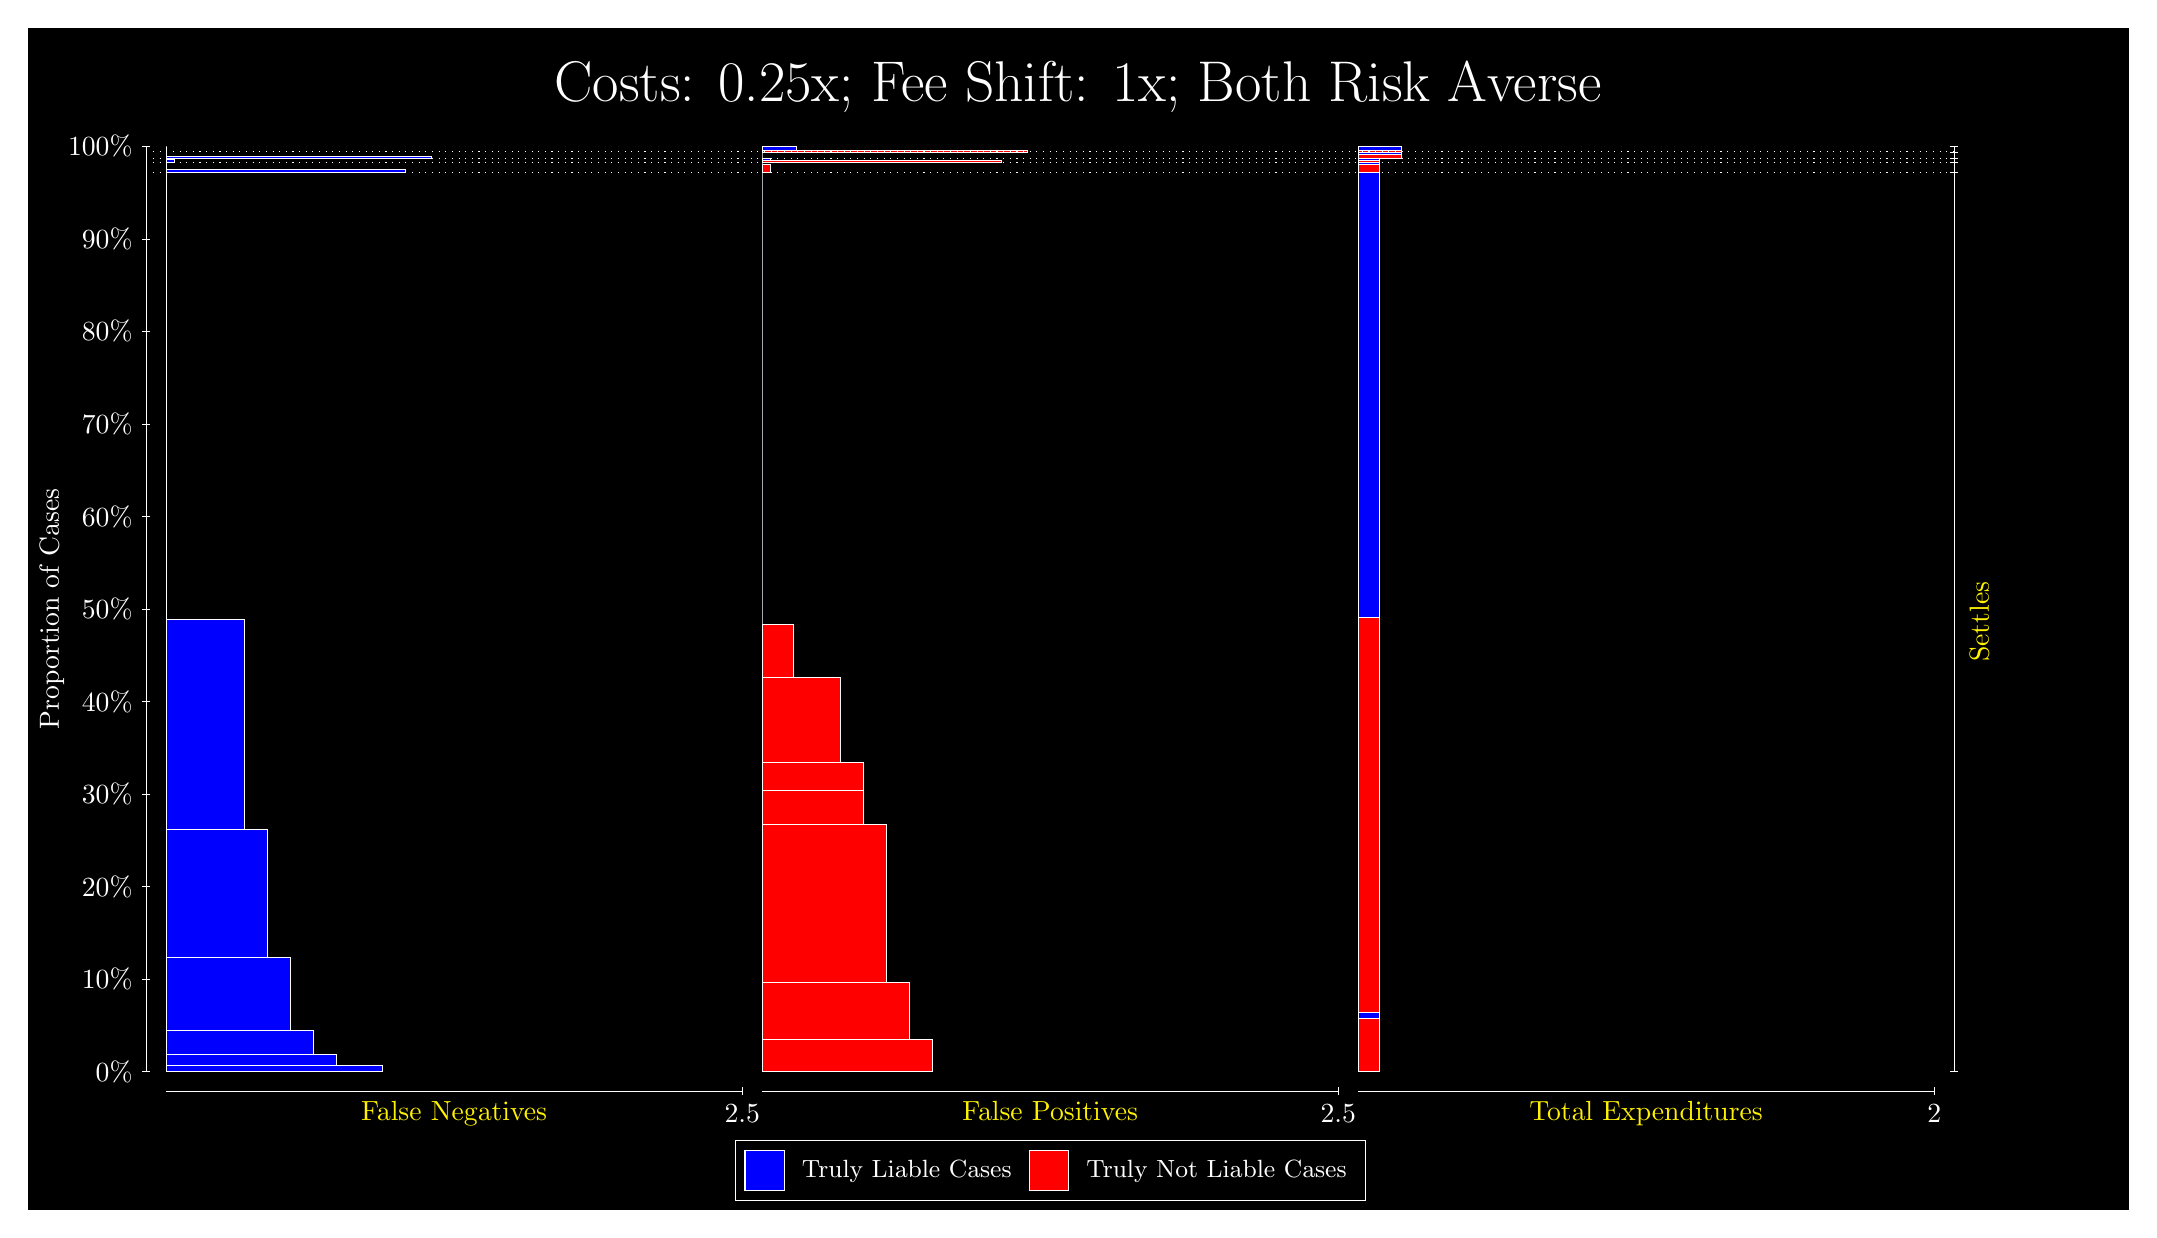
\begin{tikzpicture}
\draw[fill=black] (0,0) rectangle (26.667,15);
\draw[text=white] (0,13.5) rectangle (26.667,15) node[midway] {\huge Costs: 0.25x; Fee Shift: 1x; Both Risk Averse};
\draw[white, very thin] (1.5,1.75) -- (1.5,13.5);
\node[rotate=90, text=white, anchor=center] at (0.3, 7.625) {Proportion of Cases};
\draw[white, very thin] (1.45,1.75) -- (1.55,1.75);
\node[text=white, anchor=east] at (1.45, 1.75) {0\%};
\draw[white, very thin] (1.45,2.925) -- (1.55,2.925);
\node[text=white, anchor=east] at (1.45, 2.925) {10\%};
\draw[white, very thin] (1.45,4.1) -- (1.55,4.1);
\node[text=white, anchor=east] at (1.45, 4.1) {20\%};
\draw[white, very thin] (1.45,5.275) -- (1.55,5.275);
\node[text=white, anchor=east] at (1.45, 5.275) {30\%};
\draw[white, very thin] (1.45,6.45) -- (1.55,6.45);
\node[text=white, anchor=east] at (1.45, 6.45) {40\%};
\draw[white, very thin] (1.45,7.625) -- (1.55,7.625);
\node[text=white, anchor=east] at (1.45, 7.625) {50\%};
\draw[white, very thin] (1.45,8.8) -- (1.55,8.8);
\node[text=white, anchor=east] at (1.45, 8.8) {60\%};
\draw[white, very thin] (1.45,9.975) -- (1.55,9.975);
\node[text=white, anchor=east] at (1.45, 9.975) {70\%};
\draw[white, very thin] (1.45,11.15) -- (1.55,11.15);
\node[text=white, anchor=east] at (1.45, 11.15) {80\%};
\draw[white, very thin] (1.45,12.325) -- (1.55,12.325);
\node[text=white, anchor=east] at (1.45, 12.325) {90\%};
\draw[white, very thin] (1.45,13.5) -- (1.55,13.5);
\node[text=white, anchor=east] at (1.45, 13.5) {100\%};

\draw[white, very thin] (24.457,1.75) -- (24.457,13.5);
\draw[white, very thin] (24.407,1.75) -- (24.507,1.75);
\node[anchor=west] at (24.407, 1.75) {};
\draw[white, very thin] (24.407,13.173) -- (24.507,13.173);
\node[anchor=west] at (24.407, 13.173) {};
\draw[white, very thin] (24.407,13.297) -- (24.507,13.297);
\node[anchor=west] at (24.407, 13.297) {};
\draw[white, very thin] (24.407,13.351) -- (24.507,13.351);
\node[anchor=west] at (24.407, 13.351) {};
\draw[white, very thin] (24.407,13.429) -- (24.507,13.429);
\node[anchor=west] at (24.407, 13.429) {};
\draw[white, very thin] (24.407,13.5) -- (24.507,13.5);
\node[anchor=west] at (24.407, 13.5) {};

\draw[white, very thin, fill=blue] (1.75,1.75) rectangle (4.4946,1.8298);
\draw[white, very thin, fill=blue] (1.75,1.8298) rectangle (3.9091,1.964);
\draw[white, very thin, fill=blue] (1.75,1.964) rectangle (3.6163,2.2754);
\draw[white, very thin, fill=blue] (1.75,2.2754) rectangle (3.3236,3.195);
\draw[white, very thin, fill=blue] (1.75,3.195) rectangle (3.0308,4.8218);
\draw[white, very thin, fill=blue] (1.75,4.8218) rectangle (2.738,7.4896);
\draw[white, very thin, fill=red] (1.75,7.4896) rectangle (1.75,13.173);
\draw[white, very thin, fill=blue] (1.75,13.173) rectangle (4.7873,13.204);
\draw[white, very thin, fill=red] (1.75,13.204) rectangle (1.75,13.297);
\draw[white, very thin, fill=blue] (1.75,13.297) rectangle (1.8598,13.331);
\draw[white, very thin, fill=red] (1.75,13.331) rectangle (1.75,13.351);
\draw[white, very thin, fill=blue] (1.75,13.351) rectangle (5.1167,13.376);
\draw[white, very thin, fill=red] (1.75,13.376) rectangle (1.75,13.429);
\draw[white, very thin, fill=red] (1.75,13.429) rectangle (1.75,13.454);
\draw[white, very thin, fill=blue] (1.75,13.454) rectangle (1.75,13.5);
\draw[white, very thin, fill=red] (9.3189,1.75) rectangle (11.478,2.1641);
\draw[white, very thin, fill=red] (9.3189,2.1641) rectangle (11.185,2.8855);
\draw[white, very thin, fill=red] (9.3189,2.8855) rectangle (10.892,4.8846);
\draw[white, very thin, fill=red] (9.3189,4.8846) rectangle (10.6,5.3185);
\draw[white, very thin, fill=red] (9.3189,5.3185) rectangle (10.6,5.6754);
\draw[white, very thin, fill=red] (9.3189,5.6754) rectangle (10.307,6.762);
\draw[white, very thin, fill=red] (9.3189,6.762) rectangle (9.7214,7.4338);
\draw[white, very thin, fill=blue] (9.3189,7.4338) rectangle (9.3189,13.173);
\draw[white, very thin, fill=red] (9.3189,13.173) rectangle (9.4287,13.267);
\draw[white, very thin, fill=blue] (9.3189,13.267) rectangle (9.3189,13.297);
\draw[white, very thin, fill=red] (9.3189,13.297) rectangle (12.356,13.317);
\draw[white, very thin, fill=blue] (9.3189,13.317) rectangle (9.4287,13.351);
\draw[white, very thin, fill=red] (9.3189,13.351) rectangle (9.3189,13.403);
\draw[white, very thin, fill=blue] (9.3189,13.403) rectangle (9.3189,13.429);
\draw[white, very thin, fill=red] (9.3189,13.429) rectangle (12.686,13.454);
\draw[white, very thin, fill=blue] (9.3189,13.454) rectangle (9.758,13.5);
\draw[white, very thin, fill=red] (16.888,1.75) rectangle (17.162,2.4218);
\draw[white, very thin, fill=blue] (16.888,2.4218) rectangle (17.162,2.5016);
\draw[white, very thin, fill=red] (16.888,2.5016) rectangle (17.162,7.5136);
\draw[white, very thin, fill=blue] (16.888,7.5136) rectangle (17.162,13.173);
\draw[white, very thin, fill=red] (16.888,13.173) rectangle (17.162,13.267);
\draw[white, very thin, fill=blue] (16.888,13.267) rectangle (17.162,13.297);
\draw[white, very thin, fill=red] (16.888,13.297) rectangle (17.162,13.317);
\draw[white, very thin, fill=blue] (16.888,13.317) rectangle (17.162,13.351);
\draw[white, very thin, fill=red] (16.888,13.351) rectangle (17.437,13.403);
\draw[white, very thin, fill=blue] (16.888,13.403) rectangle (17.437,13.429);
\draw[white, very thin, fill=red] (16.888,13.429) rectangle (17.437,13.454);
\draw[white, very thin, fill=blue] (16.888,13.454) rectangle (17.437,13.5);
\draw[white, dotted] (1.5,13.173) -- (24.457,13.173);
\draw[white, dotted] (1.5,13.297) -- (24.457,13.297);
\draw[white, dotted] (1.5,13.351) -- (24.457,13.351);
\draw[white, dotted] (1.5,13.429) -- (24.457,13.429);
\draw[white, very thin] (1.75,1.5) -- (9.0689,1.5);
\node[text=yellow, anchor=north] at (5.4094, 1.5) {False Negatives};
\draw[white, very thin] (9.0689,1.45) -- (9.0689,1.55);
\node[text=white, anchor=north] at (9.0689, 1.45) {2.5};

\draw[white, very thin] (9.3189,1.5) -- (16.638,1.5);
\node[text=yellow, anchor=north] at (12.978, 1.5) {False Positives};
\draw[white, very thin] (16.638,1.45) -- (16.638,1.55);
\node[text=white, anchor=north] at (16.638, 1.45) {2.5};

\draw[white, very thin] (16.888,1.5) -- (24.207,1.5);
\node[text=yellow, anchor=north] at (20.547, 1.5) {Total Expenditures};
\draw[white, very thin] (24.207,1.45) -- (24.207,1.55);
\node[text=white, anchor=north] at (24.207, 1.45) {2};

\node[text=yellow, centered, rotate=90] at (24.777, 7.4617) {Settles};





\draw (12.978300999999998,1.5) node[draw=none] (baseCoordinate) {};
\begin{scope}[align=center]
        \matrix[scale=0.5, draw=white, below=0.5cm of baseCoordinate, nodes={draw}, column sep=0.1cm]{
            \node[rectangle, draw, minimum width=0.5cm, minimum height=0.5cm, fill=blue] {}; &
            \node[draw=none, font=\small, text=white] (B) {Truly Liable Cases}; &
            \node[rectangle, draw, minimum width=0.5cm, minimum height=0.5cm, fill=red] {}; &
            \node[draw=none, font=\small, text=white] (B) {Truly Not Liable Cases}; \\
            };
\end{scope}

\end{tikzpicture}
\end{document}